\documentclass{llncs}
\usepackage{makeidx}
\usepackage{cite}
\usepackage{graphicx}
\usepackage{amssymb}

%

\begin{document}
\pagestyle{plain}

\mainmatter

\title{Accounting for Heterogeneity Across Multiple Imaging Sites Using Multi-Task
  Learning}
%
\titlerunning{short title}  % abbreviated title (for running head)
%
% use \inst{1} to get numbered tags on authors to match affiliations
\author{No Author Given}
%\author{Michelle T. Hromatka\inst{1} \and Wei Liu\inst{1}  \and Jeffrey S. Anderson\inst{2} \and Brandon A. Zielinski\inst{3} \and Molly B. DuBray\inst{4} \and P. Thomas Fletcher\inst{1}}
\institute{No Institute given}
%\institute{School of Computing\and Division of Neuroradiology \and Division of Child Neurology\and
%Interdepartmental Program in Neuroscience
%\\ University of Utah, Salt Lake City, UT 84112, USA}

\maketitle

\begin{abstract}
Combining imaging data from multiple sites has the potential to increase
statistical power in clinical studies. However, while pooling multiple data
sources increases sample size, it also increases unwanted variance due to
inconsistencies across sites, e.g., different scanners, protocols, and
demographics. In this paper, we present an approach for combining multi-site
imaging data in classification tasks that takes this heterogeneity into
account. The idea is to treat the classification problem as a multi-task
learning problem, where each imaging site is treated as a ``task''. We employ a
regularized support vector machine (SVM) that allows for differences in decision
boundaries at individual sites, while at the same time leveraging the
similarities in the decision boundaries across sites. We demonstrate the
effectiveness of this approach in the classification of autism from multi-site
functional magnetic resonance imaging (fMRI) from the Autism Brain Imaging Data
Exchange (ABIDE). The proposed method achieves state-of-the-art accuracy and
outperforms a comparable SVM classifier applied to pooled data as well as
individual SVM classifiers applied per site.

% This paper combines traditional learning methods with regularized multi-task learning  to account for the differences between site data while still assuming similarity between tasks.  The ABIDE dataset is used for this research where a third of the data are removed and used to select a variety of parameters which are then used within a leave-one-out SVM classifier for the remaining test subjects. \keywords{SVM classification, ABIDE, Autism, ASD, multi-task learning, multi-site data }
\end{abstract}

\section{Introduction}
Recent years have seen a movement towards combining neuroimaging data collected
across multiple sites. Such multi-site data has the potential to accelerate
scientific discovery by increasing sample sizes, providing broader ranges of
participant demographics, and making data publicly available. Different
approaches include large, coordinated multi-site neuroimaging studies, such as
the Alzheimer's Disease Neuroimaging Initiative (ADNI) \cite{adni}, as well as
data sharing initiatives that combine multiple single-site studies, such as the
Autism Brain Imaging Data Exchange (ABIDE) \cite{abide}. Analysis using these
datasets, however, is not straightforward, due to differences across site
scanners, protocols, populations, and diagnosis techniques. Treating a
multi-site study as a single, homogeneous data set fails to account for this
variability, which can be detrimental to the statistical power and counteract
the gains made by increasing the sample size.

An alternative approach is to perform separate statistical analyses at
individual sites and combine the results in a meta-analysis. This is often
formulated as a random effects model~\cite{DerSimonian}, where each site is
regarded as a random treatment effect. While this can be an effective way to
combine statistical tests of low-dimensional summary measures, it is less
applicable to learning problems on high-dimensional data such as images. For
instance, applying independent classifiers at each site and then combining them
post-hoc misses the opportunity that the classifiers could benefit from sharing
information across sites during learning.  Meta-analysis is also prone to publication bias, meaning only results from 
studies whose results were significant enough to publish are aggregated.  By using shared raw data instead of widely 
published results, this bias can ideally be avoided \cite{meta}. 

In this paper, we propose an approach for combining multiple imaging studies in
classification problems. The idea is to treat the problem as a multi-task
learning problem, where classifiers for each site are estimated jointly, with a
regularization that favors similarity across sites. This allows classifiers to
share information during learning, but also provides the flexibility for them to
differ at each site as needed. This is the key principle in multi-task learning:
heterogeneity across similar tasks (or, in our case, sites) can be accounted for
while using a common mean to account for similarities between the different
tasks. We specifically employ a regularized support vector machine (SVM)
introduced by Evgeniou and Pontil~\cite{regMTL}. As a driving problem, we
apply this method to the classification of autism from functional magnetic
resonance imaging (fMRI) from the ABIDE database.

Several groups have reported classification results using the ABIDE data, in
each case treating the pooled collection of images across all sites as a single
homogeneous dataset during classification. Nielsen, et al.~\cite{Jared} combines
the ABIDE dataset with a whole-brain approach, using a leave-one-out classifier
to compute a classification score for each left-out subject based on age, gender
and handedness. The correlations for each connection in turn were fit with a
linear model, separating controls from subjects with an Autism Spectrum Disorder (ASD), which was then adjusted by the
difference between the subject's site mean for that connection and the overall
mean. This approach yielded a maximum overall accuracy of 60.0\% despite finding
significant positive correlation between the classification score and several of
the phenotypic behavioral measures \cite{Jared}. A different study used
histogram of gradients and applied this to several multi-site imaging studies
which was able to achieve 61.7\% accuracy on the ABIDE dataset and 62.6\% on the
ADHD-200 dataset \cite{ghiassian}. While \cite{Jared} accounted for the site
differences during feature generation and selection, both studies approached the
differences across imaging sites as noise instead of extra data that can be
leveraged when classifying an aggregate data set.

% Many researchers fail to take these differences as a****8, but rather as increased noise when treating with the drawback of increased noise due to scanner, protocol and population differences.}
  
%Previous efforts to combine single-site studies have relied primarily on meta-analysis, in which results across small sites are statistically combined to extract patterns common across the combined sample size. Meta-analysis, however, is not free of subjectivity of data variability, thus this method of combined analysis is also faulty \cite{meta}.

\section{Methods}
Classification of multi-site imaging data can be thought of as a multi-task learning problem where each site,  $s$, is treated as a separate task, $t$.  For a dataset with $S$ sites, the corresponding multi-task problem will have a set of $T = S$ tasks and a function $F(t)$ that describes the relationship between each task.
Prior to using any sort of machine learning, however, nuisance factors (e.g. age) should be ***removed? from the data to ideally isolate differences across all data that are exclusive to the ***disease, disorder?**** being studied.

% SVM parameters through cross-validation and the features to be used in classification (see \ref{subsec:FS}).  These parameters are then used in a leave-one-out classifier on the testing data to determine the algorithm's accuracy, sensitivity and specificity. It is important to note that all parameter tuning and feature selection is done exclusively on the \textit{training} set, and the testing set is only used in the final classification to avoid inflation of results.

\subsection{Multi-Task Learning}
\label{subsec:MTL}
Evgeniou and Pontil~\cite{regMTL} introduce a method of multi-task learning based on kernel methods typically used for single task learning.  This method relies on minimizing regularization functions, such as that for SVM, to capture both overall similarity between tasks and individual task differences.  The traditional minimization for a soft margin SVM is
\begin{equation}
\label{eq:svm}
\frac{1}{2}w^2 + C F\left(\sum_{i=1}^t \xi_i\right),
\end{equation}
where $C$ is a constant and $F(\mu)$ is a monotonic convex function with $F(0)=0$ \cite{svm}. In the case of SVMs, the weight vector $w$ is used to define the hyperplane, $(w \cdot x +b)$,  which is the boundary between groups.

For multi-task learning, the relationship between $T$ tasks must be described, which can be framed as a hierarchical model. This assumes that each task function comes from a class of probability distributions.  The relationship is defined as\\
\begin{equation}
\label{eq:sim}
 w_t = w_0 + v_t ,
\end{equation}
where $w_0$ is the mean of the data and each task $t$ has its own weight vector, $v_t$. Multi-task learning allows for simultaneous learning of the mean of all tasks, $w_0$, and each task weight vector, $v_t$, so the minimization function then becomes\\
\begin{equation}
\label{eq:mtlsvm}
 C \sum_{t=1}^T \sum_{i=1}^m \xi_{it} + \frac{\lambda_1}{T} \sum_{t=1}^T ||v_t||^2 + \lambda_2||w_0||^2 ,
\end{equation}
where $\lambda_1, \lambda_2$ are positive regularization parameters, and $C$ is still a constant. For high similarity between tasks, the $v_t$ will be small in relation to $w_0$; this relationship is described by the hyperparameters $\lambda_1, \lambda_2$ that must be chosen by the user.

The dual of equation \ref{eq:mtlsvm} can be found by defining a set of functions $f_t(x) = w_t \cdot x$ which can be simplified to $F(x,t) = f_t(x)$.  This can be described by a kernel function $\phi((x,t))$ which allows us to relate the dual of a multi-task learning problem to the dual of Equation \ref{eq:svm}.
\begin{equation}
\label{eq:mtldual}
\max_{\alpha_{it}}  \left\{ \sum_{i=1}^m\sum_{t=1}^T \alpha_{it} -  \sum_{i=1}^m\sum_{s=1}^T\sum_{j=1}^m\sum_{t=1}^T  \alpha_{is}y_{is}\alpha_{jt}y_{jt}\phi((x,t))      \right\}
\end{equation}
where
\begin{equation}
\phi((x,t)) = \big(\frac{x}{\sqrt{\mu}}, \underbrace{0,...,0}_{t-1}, x, \underbrace{0,...,0}_{T-t} \big), \quad \textbf{for  } \mu = \frac{T\lambda_2}{\lambda_1} .
\end{equation}
As you can see in Equation \ref{eq:mtldual}, this is the same dual problem as for a single task-SVM, with the data transformed by $\phi((x,t))$ into the multi-task kernel space.




\subsection{Feature Selection}
\label{subsec:FS}
Data extraction in imaging studies typically leads to very high dimensional data spaces.  For f-MRI, a typical choice for data is the pairwise correlation between $n$ predefined regions of the brain.  This yields a dataspace of $\frac{n(n+1)}{2}$ dimensionality, which, even for a relatively small number of regions, can be  computationally expensive.  The multi-task learning above further increases dimensionality with the number of tasks. For a feature space $x \in \mathbb{R}^d$, the multi-task kernel $\phi((x,t))$ would yield a feature space of $d(t+1)$ dimensions.  Feature selection can and should be employed to remove redundancy and increase relevancy of the data while reducing computation time \cite{featsel}.


One approach is to use the values of the weight vector $w$ to choose the most relevant features.  Recall that the decision boundary in an SVM is defined by $w \cdot x$, meaning the highest magnitudes in the weight vector denote the features that best define the decision boundary between groups. This is the basis for the SVM recursive feature elimination(SVM-RFE) method demonstrated in \cite{guyon2002gene}, \cite{abide}, \cite{ecker2010} where a user-specified number of features corresponding to the lowest $w$ values are removed from the feature set each iteration. We modify SVM-RFE to rank by region, instead of by individual pairwise correlation, effectively reducing the data dimension for feature selection purposes while still leveraging the correlation data. 
%A ****** approach is to use a simple hypothesis test to determine which features would be most useful in classification.  Nuisance factors, such as age or ******, should be accounted for prior to the hypothesis test to ideally isolate differences attributed to the disease or disorder being studied.  A linear model is then fit to the training set one feature at a time based on group.  If the coefficient for the group  has a $p < .001$, the feature is kept and used in the SVM classification. This test is done on each feature in turn, ultimately reducing the data into a set that has significant differences between groups.
\section{Evaluation}
\subsection{Data}
The Autism Brain Imaging Data Exchange(ABIDE) database is an online consortium of resting-state functional-MRI data from 17 international sites, resulting in brain imaging data for 539 individuals with ASD and 573 typically developing(TD)  controls \cite{abide}. All ASD subjects were diagnosed by either the Autism Diagnosis Observation Schedule-General(ADOS-G) or the Autism Diagnostic Interview-Revised tests and removed from the study if other co-morbid disorders were present \cite{lordADOS} \cite{lordADIR} \cite{abide}.  Further inclusion details can be found at (put url? citation to... website? or the abide paper?)
\subsubsection{Preprocessing}
All data was preprocessed using the Functional Connectomes-1000 preprocessing scripts \cite{fcon}. This includes:
\begin{enumerate}
\item MRI Deoblique, reorient, skull strip
\item f-MRI Reorient, motion correct, skull strip, smooth
\item registration
\item Segmentation - csf, white matter
\item extracting global signal, from csf and wm
\item extract time series, Z-transform correlations
\item spatial smoothing, register to atlas
\item some sort of regression
\end{enumerate}
Twelve subjects were removed because of failure during the preprocessing.  Two Oregon subjects were missing the resting fMRI file and 10 UCLA subjects were missing the anatomical scan file which is required in step 1 of the preprocessing pipeline above. This resulted in 1100 subjects for analysis, 530 ASD and 570 TD controls.
\subsubsection{Data Extraction}
From each subject's postprocessed image, the time series for each of 264 regions is extracted based on Power's regions of interest \cite{Powers}. These 264 regions are spread out among the cerebral cortex, subcortical structures and cerebellum, where each region is a sphere of 5mm in radius and regions are separated by a minimum distance of 10mm so as to avoid detection of a shared signal. The Fisher transformed Pearson correlation coefficient is then found between each region and all other 263 regions, resulting in a 34,716 dimensional feature space for each subject. After feature selection, this number was reduced to ****** regions of the original 264, yielding a final dimensionality of ***** features
\subsection{Results}
The ABIDE data was split into two sets; one half of the data was used for training, the other half was used exclusively to test our approach.  This divide was first done at the site level, a random division within ASD and controls, to preserve the ratios between sites and groups across the two data sets.

We present results for three cases: one where each site was classified individually, a second where all site data was pooled and considered a single site and the third using the multi-task learning approach described in \ref{subsec:MTL}. For all of the results presented within, a radial basis function (RBF) kernel was used in the SVM, with parameters $C$ and $\gamma$ determined by cross validation on the training set. Multi-task learning requires an additional parameter, $\mu$, used to control similarity across tasks; this was also determined during cross validation. The training set was also used to determine nuisance factor regression on subject age, and feature selection for use on the testing set prior to the leave one out classifier.  ***All values determined by the training set were fixed across each experiment in order to test the difference between the classification cases, not the effectiveness of parameter tuning.

% If don't have time for CV with mu
%For multi-task learning, the results are presented with varying values of $\mu$.  Recall that $\mu$ is defined as $\frac{T\lambda_2}{\lambda_1}$, which is used to compute the mean across all tasks, $w_0$, in the formulation of $\phi((x,t))$. For very small values of $\mu$, the $w_0$ term becomes very large in relation to each task's individualized weight vector, $v_t$, so the problem essentially becomes a single-task learning problem.  The converse, where $\mu$ is very large, approaches the scenario where the tasks are completely unrelated \cite{regMTL}. 
%This can be seen in figure ******, where a $mu$ value of ***** corresponds to single task learning and a $mu$ value of ****** corresponds to classifying each task individually.  The ******* indicate our results for single-task learning and the combined accuracy for individual task classification.
%The ideal value for $\mu$ appears to be at ********, where the accuracy reaches a peak of ********.

The multi-task learning approach is significantly better than the single task approach, which is in turn much better than the individual task approach. A caveat is that the sensitivity and specificity values for single task learning seem to be more stable***?? than in the multi-task result. 
\begin{figure}
	\centering
	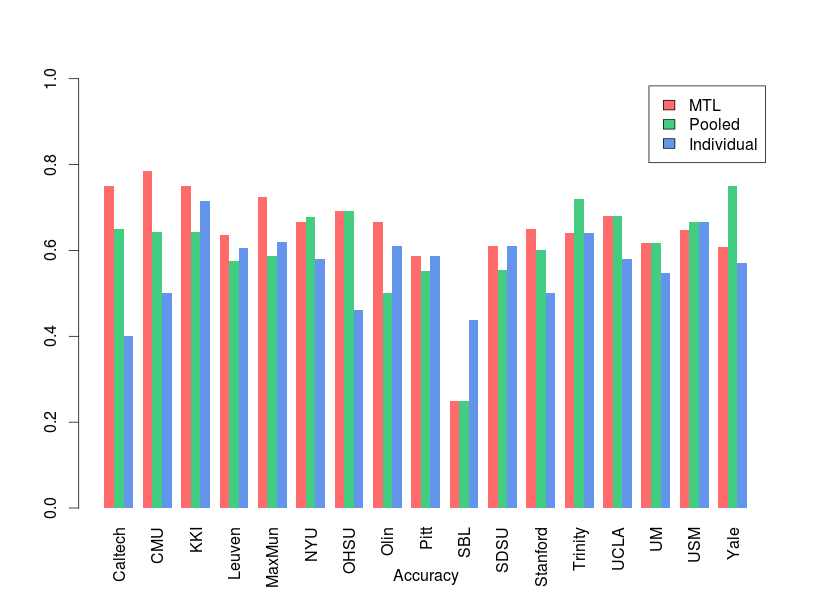
\includegraphics[scale = .6]{acc_bar.png}
	\caption{The overall accuracies by site, as found by each of the three experiments. }
	\label{fig:acc_bar}
\end{figure}


Several datasets benefited greatly from the increase in data size, increasing **************.  For sites that were relatively stable to begin with because of sample size, the MTL approach did not find a large improvement to that sites overall accuracy.
 
\section{Discussion and Conclusion}
\begin{figure}
	\centering
	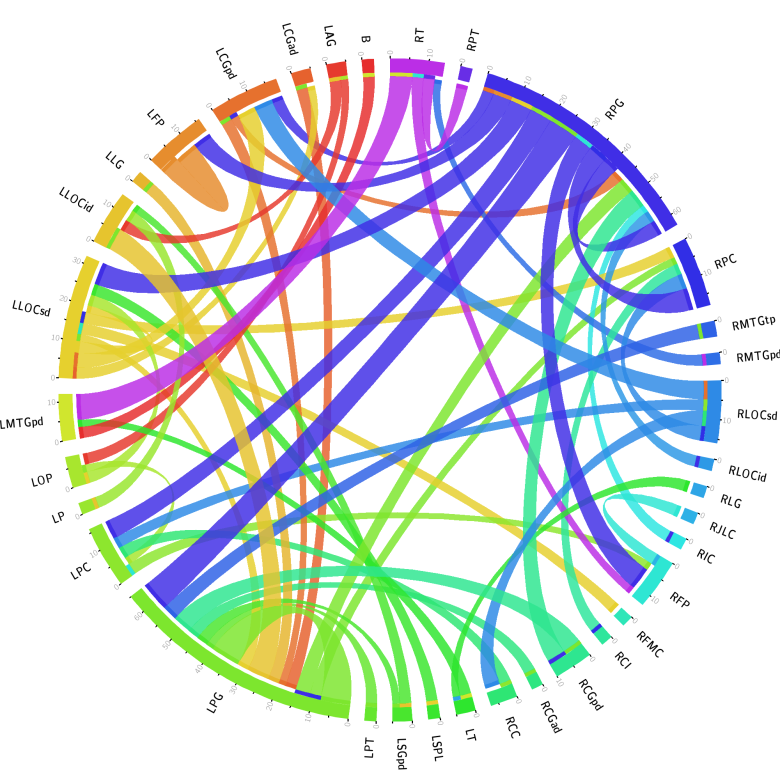
\includegraphics[scale = .3]{now_circos.png}
	\caption{The pairwise connections, represented as ribbons connecting each region, selected by the hypothesis test described in \ref{subsec:FS}.  The width of each ribbon is determined by the weights from the $w_0$ vector in the SVM. }
	\label{fig:circos}
\end{figure}

Figure \ref{fig:circos} displays the regions identified via the method described \ref{subsec:FS}.  The regions show a strong overlap with ROIs previously identified as network “hubs” thought to be abnormal in autism, namely the default mode network and socioemotional salience network.  Atypical network structure and function, identified in structural covariance MRI \cite{zielinski2012scmri} and also functional connectivity studies (reviewed in \cite{jeff2014}), may contribute to many of the behaviors associated with the disorder.



\bibliography{miccai}{}
\bibliographystyle{plain}





\end{document}